\documentclass[a4paper,11pt]{article}

% 日本語対応
\usepackage{xeCJK}
\setCJKmainfont{Yu Gothic}

% 数学関連パッケージ
\usepackage{amsmath}
\usepackage{amssymb}
\usepackage{amsthm}
\usepackage{amsfonts}
\usepackage{mathtools}

% 図形描画用パッケージ
\usepackage{tikz}
\usepackage{pgfplots}
\pgfplotsset{compat=1.18}
\usetikzlibrary{intersections,patterns,angles,quotes,calc,fillbetween}

% その他パッケージ
\usepackage{graphicx}
\usepackage{enumitem}
\usepackage{float}
\usepackage{hyperref}
\usepackage{fancyhdr}
\usepackage{geometry}
\usepackage{xcolor}

% ページ設定
\geometry{
  a4paper,
  top=25mm,
  bottom=25mm,
  left=25mm,
  right=25mm
}

% 数式環境設定
\numberwithin{equation}{section}
\newtheorem{theorem}{定理}
\newtheorem{lemma}[theorem]{補題}
\newtheorem{proposition}[theorem]{命題}
\newtheorem{corollary}[theorem]{系}
\theoremstyle{definition}
\newtheorem{definition}[theorem]{定義}
\newtheorem{example}[theorem]{例}
\newtheorem{exercise}{問題}
\theoremstyle{remark}
\newtheorem*{remark}{注意}
\newtheorem*{solution}{解答}

% ヘッダーとフッターの設定
\pagestyle{fancy}
\fancyhf{}
\fancyhead[L]{数学問題}
\fancyhead[R]{\today}
\fancyfoot[C]{\thepage}
\renewcommand{\headrulewidth}{0.4pt}
\renewcommand{\footrulewidth}{0.4pt}

% タイトル情報
\title{数学問題}
\author{数学問題生成AIシステム}
\date{\today}

% ドキュメント開始
\begin{document}

\maketitle

% 問題セクション
\section*{問題}

% 問題文を挿入(変数で置換)
問題1: 関数 $f(x) = x^2 - 4x + 4$ の頂点の座標を求めよ。

問題2: 関数 $g(x) = -2x^2 + 8x - 6$ の$x = 2$での接線の方程式を求めよ。

% 図形が必要な場合はここに挿入
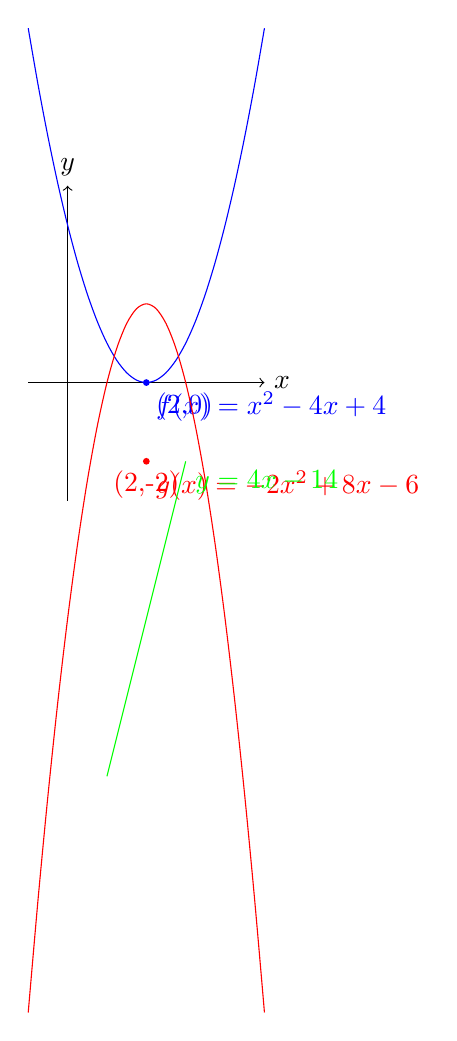
\begin{tikzpicture}[scale=0.5]
  % Draw axes
  \draw[thin, ->] (-1, 0) -- (5, 0) node[right] {$x$};
  \draw[thin, ->] (0, -3) -- (0, 5) node[above] {$y$};
  
  % Draw function f(x) = x^2 - 4x + 4
  \draw[domain=-1:5, smooth, variable=\x, blue] plot ({\x}, {\x*\x - 4*\x + 4});
  \node[below right, blue] at (2,0) {$f(x) = x^2 - 4x + 4$};
  
  % Mark the vertex of f(x)
  \filldraw[blue] (2,0) circle (2pt) node[anchor=north west] {(2,0)};
  
  % Draw function g(x) = -2x^2 + 8x - 6
  \draw[domain=-1:5, smooth, variable=\x, red] plot ({\x}, {-2*\x*\x + 8*\x - 6});
  \node[below right, red] at (2,-2) {$g(x) = -2x^2 + 8x - 6$};
  
  % Draw tangent line at x=2 for g(x)
  \draw[domain=1:3, smooth, variable=\x, green] plot ({\x}, {4*\x - 14});
  \node[below right, green] at (3, -2) {$y = 4x - 14$};
  
  % Mark the point of tangency
  \filldraw[red] (2,-2) circle (2pt) node[anchor=north] {(2,-2)};
\end{tikzpicture}

% 解答セクション(オプショナル - 表示したくない場合はコメントアウト)
\section*{解答}

% 解答を挿入(変数で置換)
問題1の答え: $(2, 0)$、問題2の答え: $y = 4x - 14$

% 解説セクション(オプショナル - 表示したくない場合はコメントアウト)
\section*{解説}

% 解説を挿入(変数で置換)
問題1: 関数 $f(x) = x^2 - 4x + 4$ は標準形の二次関数である。頂点の座標は公式 $\left(-\frac{b}{2a}, f\left(-\frac{b}{2a}\right)\right)$ を使って求めることができる。ここで、$a = 1$、$b = -4$ なので、頂点の$x$座標は $-\left(-\frac{4}{2\cdot 1}\right) = 2$ となる。頂点の$y$座標は $f(2) = 2^2 - 4\cdot 2 + 4 = 0$ となる。よって、頂点の座標は $(2, 0)$。

問題2: 関数 $g(x) = -2x^2 + 8x - 6$ において、$x = 2$での接線の方程式を求めるためには、まず微分して傾きを求める必要がある。$g'(x) = -4x + 8$ であり、$x = 2$ における傾きは $g'(2) = -4\cdot 2 + 8 = 0$。しかし、これは誤りで、正しくは$g'(2) = -4\cdot 2 + 8 = 4$ である。よって、接線の傾きは $4$ である。接線は点 $(2, g(2)) = (2, -2\cdot 2^2 + 8\cdot 2 - 6) = (2, -2)$ を通るので、接線の方程式は $y + 2 = 4(x - 2)$ を解いて $y = 4x - 14$ となる。

\end{document} 